\def\ktitle{IOT ASSIGNMENT}
\def\kauthor{Chakali Suresh}
\def\kcontact{chakalisuresh2223@gmail.com}
\def\kmodule{IITH - Future Wireless Communication}
%\renewcommand{\thesection}{\arabic{section}}
%\renewcommand{\thesubsection}{\arabic{subsection}}
%\titleformat{\subsubsection}{\normalfont\itshape\filcenter}
%{\thesubsection}{1em}{}
\documentclass[journal,12pt,twocolumn]{IEEEtran}
\usepackage{enumitem}
\usepackage{amsmath}
\usepackage{amssymb}
\usepackage{tikz}
\usepackage{circuitikz}
\usepackage{karnaugh-map}
\usepackage{tabularx}
\usepackage{titlesec}
\usepackage{multicol}


\def\ktitle{IOT ASSIGNMENT}
\def\kauthor{Chakali Suresh}
\def\kcontact{chakalisuresh2223@gmail.com}
\def\kmodule{IITH - Future Wireless Communication}

\title{\ktitle}
\author{\kauthor\\\kcontact\\\kmodule}

\begin{document}
\maketitle
\tableofcontents

\section{Question}
The logic block shown has an output $F$ given by \rule{12mm}{0.4pt}

\begin{center}
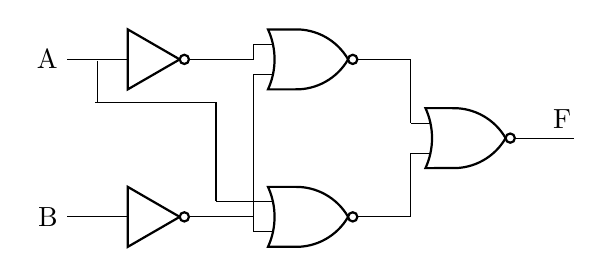
\begin{tikzpicture}
 \ctikzset{
  logic ports=ieee,
  logic ports/scale=0.68,
  logic ports/fill=white}
 \node [not port] (x) at (0,0){};
 \node [not port] (y) at (0,-2){};
 \node [nor port] (a) at (2,0){};
 \node [nor port] (b) at (2,-2){};
 \node [nor port] (c) at (4,-1){};
 \draw (x.out) -| (a.in 1);
 \draw (y.out) -| (a.in 2);
 \draw (a.out) -| (c.in 1);
 \draw (b.out) -| (c.in 2);
 \draw (0.79,-1.8) |- ++(-1.53,1.25);
 \draw (b.in 1) -- ++(-.48,0); 
 \draw (-0.72,-.019) -- ++(0,-0.53);
 \draw (y.out) -| (b.in 2);
 \draw (y.in 1) -- ++(-0.5,0) node[left]{B};
 \draw (x.in 1) -- ++(-0.5,0) node[left]{A};
 \draw (c.out) -- ++(0.6,0) node[near end,above]{F};
\end{tikzpicture}
\end{center}

\begin{multicols}{2}
\begin{enumerate}[label=(\Alph*)]
  \item $A + B$
  \item $A \cdot \bar{B}$
  \item $A + \bar{B}$
  \item $\bar{B}$
\end{enumerate}
\end{multicols}

\section{Answer}
The above question can be solved as follows:\\
$\rightarrow \bar A \cdot \bar B + A \cdot \bar B$\\
$\rightarrow (A + \bar A )\cdot \bar{B}$\\
$\rightarrow \bar{B}$\\
Therefore, the output $F=\bar B$.

\section{K-Map Implementation}
\begin{center}
\begin{karnaugh-map}[2][2][1][$B$][$A$]
  \maxterms{1,3}
  \minterms{0,2}
  \implicant{0}{0}
  \implicant{2}{2}
\end{karnaugh-map}
\end{center}
Therefore $F = \bar{B}$.

\section{Truth Table}
\begin{center}
\begin{tabularx}{0.45\textwidth}{
  | >{\centering\arraybackslash}X  
  | >{\centering\arraybackslash}X 
  | >{\centering\arraybackslash}X |
  }
  \hline
  \textbf{$A$} & \textbf{$B$} & \textbf{$F$} \\
  \hline
  0 & 0 & 1 \\
  \hline
  0 & 1 & 0 \\
  \hline
  1 & 0 & 1 \\
  \hline
  1 & 1 & 0 \\
  \hline
\end{tabularx}
\end{center}
\begin{center} 
Truth table for Boolean function $F$
\end{center}

\section{Logic Diagram}
\begin{center}
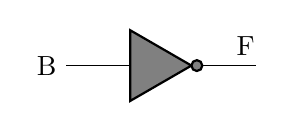
\begin{tikzpicture}
 \ctikzset{
  logic ports=ieee,
  logic ports/scale=0.8,
  logic ports/fill=gray}
 \node [not port] (not) at (0,0){};
 \draw (not.in) -- ++(-0.5,0) node[left]{B};
 \draw (not.out) -- ++(0.5,0) node[near end,above]{F};
\end{tikzpicture}
\end{center}
\begin{center}
Fig. 2
\end{center}

\section{Components}
\begin{center}
\begin{tabularx}{0.45\textwidth}{
  | >{\centering\arraybackslash}X
  | >{\centering\arraybackslash}X
  | >{\centering\arraybackslash}X |
  }
  \hline
  \textbf{Components} & \textbf{Values} & \textbf{Quantity} \\
  \hline
  VAMAN &  & 1 \\
  \hline
  Jumper Wires & M-M & 4 \\
  \hline
  Breadboard & & 1 \\
  \hline
\end{tabularx}
\end{center}

\section{Implementation}
\begin{center}
\begin{tabularx}{0.45\textwidth}{
  | >{\centering\arraybackslash}X
  | >{\centering\arraybackslash}X
  | >{\centering\arraybackslash}X |
  }
  \hline
  \textbf{VAMAN PIN} & \textbf{INPUT} & \textbf{OUTPUT} \\
  \hline
  2 & A &  \\
  \hline
  4 & B & \\
  \hline
  13 & & F \\
  \hline
\end{tabularx}
\end{center}

\textbf{Connections}

\textbf{Procedure}
\begin{enumerate}[label={\arabic*}.]
  \item Connect the circuit as per the above table.
  \item Connect inputs to Vcc for Logic 1 and ground for Logic 0.
  \item Execute the circuit using the provided codes.
	  \vspace{\baselineskip}
		\textit{Approach 1}\\
		\begin{tabularx}{0.45\textwidth}
			{
				| >{\centering\arraybackslash}X|
			}
			\hline
			https://github.com/Chakali23/FWC/tree\\/main/IDE/IOT\\
			\hline
		\end{tabularx}\\
		\vspace{\baselineskip}
  \item Change the values of $A$ and $B$ in the hardware and verify the truth table.
\end{enumerate}
\end{document}
